\chapter{Экспериментальная проверка}

\section{Условия эксперимента}
\begin{itemize}
	\item
		Проверка работы созданного прототипа осуществлялась в мае 2012 года на прямом тестовом участке длиной около 400 метров, проходящем по Покровскому и Яузскому бульварам в Москве (см. рис. \ref{fig:gfront});
	\item
		В качестве мобильного устройства использовался HTC Hero под управлением ОС Android 2.2 (см. рис. \ref{fig:tatmon-android});
	\item
		Сервер был запущен на VPS vkphoto.auditory.ru под управлением дистрибутива Gentoo ОС GNU/Linux версии 2.6.28-vs2.3.0.36.4-gentoo-ws0 с интерпретатором Python версии 2.6.4;
	\item
		Передача данных от мобильного устройства серверу по протоколу UPD осуществлялась через порт 31415;
	\item
		Входящие соединения TCP для передачи данных клиентам сервер принимал через порт 31416.
\end{itemize}

\section{Сбор данных}
Данные собирались в течение часа, по возможности равномерным образом по всей длине маршрута. В ходе эксперимента выяснился факт сравнительно редкого обновления данных GPS под Android, поэтому во время перемещения по маршруту передача данных выключалась до тех пор, пока показания широты и долготы не поменяются, затем включалась заново. Дополнительно осуществлялся контроль правильности обработки данных о местоположении путём визуального сравнения показаний клиентского приложения (см. рис. \ref{fig:gfront}\subref{subfig:gfront-gps-mode}), запущенного на портативном компьютере, подключённым к сети Интернет через общий канал с мобильным устройством, с фактической обстановкой вокруг. Координаты тестового маршрута отражены в таблице \ref{tab:exp-route-begend}. Общая статистика собранных данных отражена в таблице \ref{tab:exp-collect-data}.
\begin{table}
	\caption{\label{tab:exp-route-begend}Координаты крайних точек тестового прямого маршрута.}
	\begin{center}
		\begin{tabular}{|p{0.3\linewidth}|p{0.3\linewidth}|p{0.3\linewidth}|}
			\hline
			Точка & Широта, градусов & Долгота, градусов \\
			\hline
			Начало & 55.752361111111114 & 37.64678333333333 \\
			\hline
			Конец & 55.755430555555556 & 37.64849722222222 \\
			\hline
		\end{tabular}
	\end{center}
\end{table}

\begin{table}
	\caption{\label{tab:exp-collect-data}Статистика по собранным данным во время экспериментальной проверки системы.}
	\begin{center}
		\begin{tabular}{|p{0.8\linewidth}|p{0.1\linewidth}|}
			\hline
			Всего замеров уровней сигнала & 22675 \\
			\hline
			Замеров с различающимися значениями $<CID, Dist, RSSI>$ & 10020 \\
			\hline
			Всего различных базовых станций & 22 \\
			\hline
			Время сбора данных & 1 час \\
			\hline
		\end{tabular}
	\end{center}
\end{table}




\section{Позиционирование}
Рассмотрим трассировку процесса позиционирования, осуществлённого после сбора данных с произвольно выбранным сообщением от мобильного устройства.

\subsection{Входные данные}
Было выбрано следующее сообщение:

\lstset{language=Python}
\begin{lstlisting}
{
	"GSM":{
		"cellcount":6,
		"cells": [
				{
					"CID":41526,
					"Psc":-1,
					"RSSI":21,
					"type":"EDGE"
				},
				{
					"CID":32778,
					"Psc":-1,
					"RSSI":28,
					"type":"EDGE"
				}, 
				{
					"CID":32777,
					"Psc":-1,
					"RSSI":20,
					"type":"EDGE"
				}, 
				{
					"CID":12056,
					"Psc":-1,
					"RSSI":18,
					"type":"EDGE"
				},
				{
					"CID":14296,
					"Psc":-1,
					"RSSI":20,
					"type":"EDGE"
				},
				{
					"CID":32779,
					"Psc":-1,
					"RSSI":15,
					"type":"EDGE"
				}
			]
	}, 
	"GPS": {
		"lng":37.647523283958435,
		"ltd":55.7536518573761,
		"acc":16.0
		}
}
\end{lstlisting}

По данным класса TransRoute, расстояние от начала маршрута до проекции этой точки составляет 165,5 метров.

\subsection{Выборка собранных данных}
На этом этапе для всех имеющихся в массиве cells базовых станций осуществляется выборка ранее измеренных значений из базы данных. Графики этих значений, для каждой станции по отдельности, изображены на рис. \ref{fig:exp-cell-raw}.

\begin{figure}[p]
	\begin{center}
		\begin{subfigure}[b]{1\textwidth}
			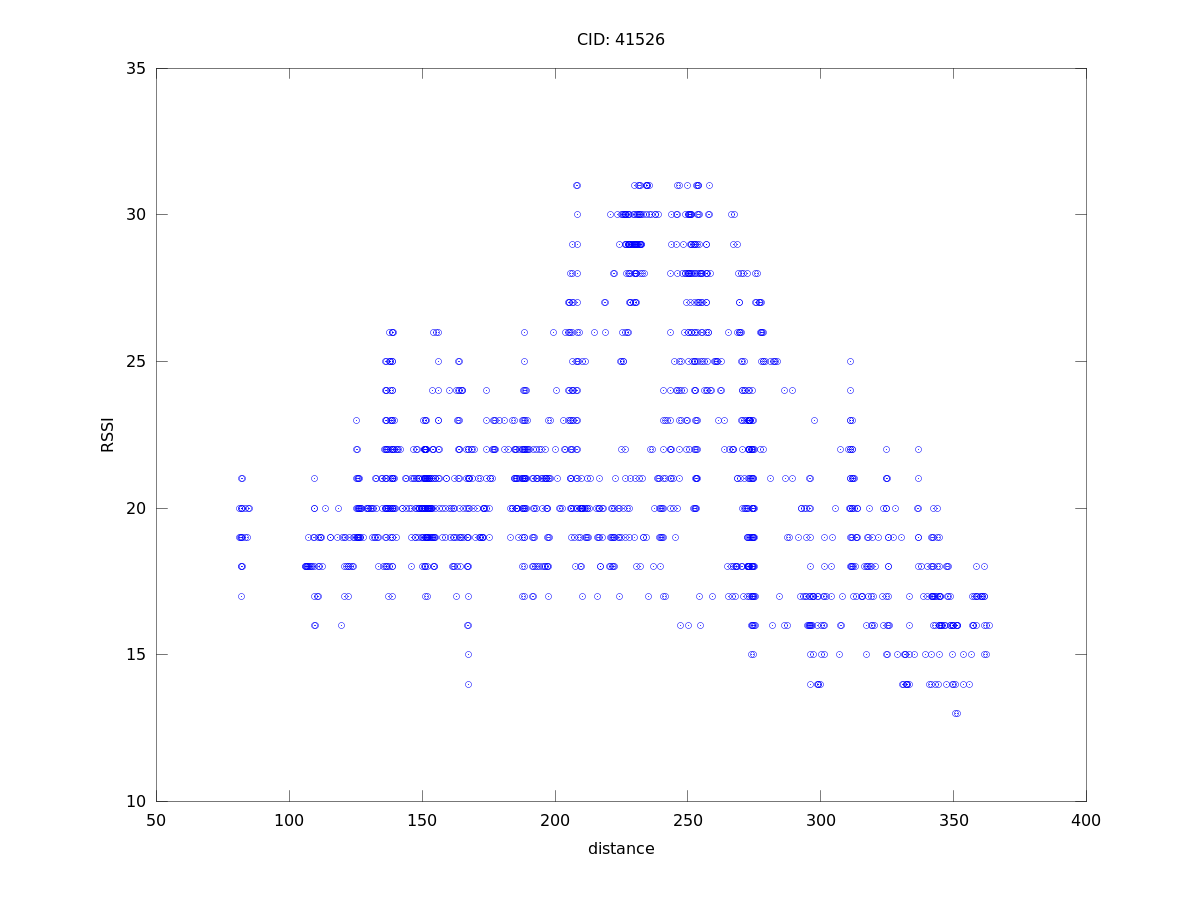
\includegraphics[width=1\textwidth]{cell41526raw.png}
		\end{subfigure}

		\begin{subfigure}[b]{0.45\textwidth}
			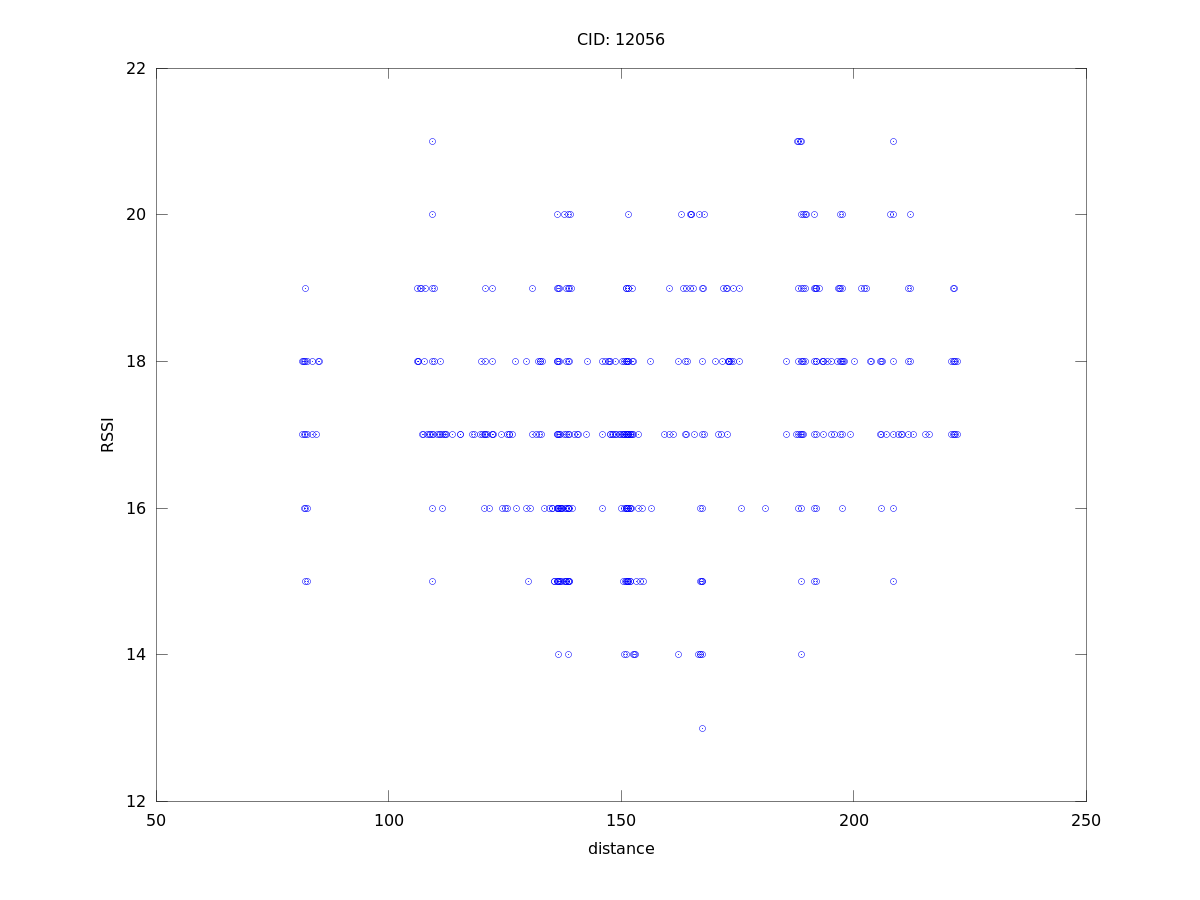
\includegraphics[width=1\textwidth]{cell12056raw.png}
		\end{subfigure}
		\begin{subfigure}[b]{0.45\textwidth}
			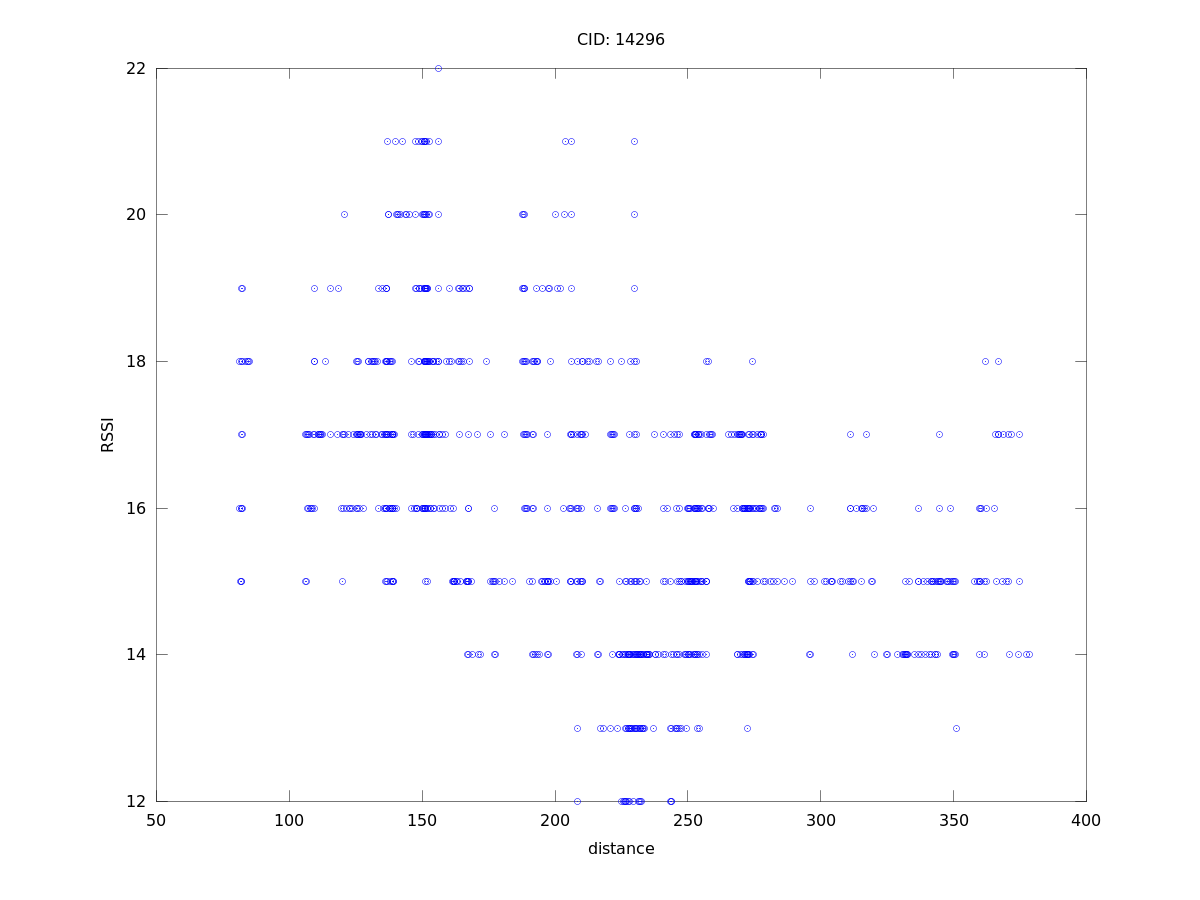
\includegraphics[width=1\textwidth]{cell14296raw.png}
		\end{subfigure}

		\begin{subfigure}[b]{0.3\textwidth}
			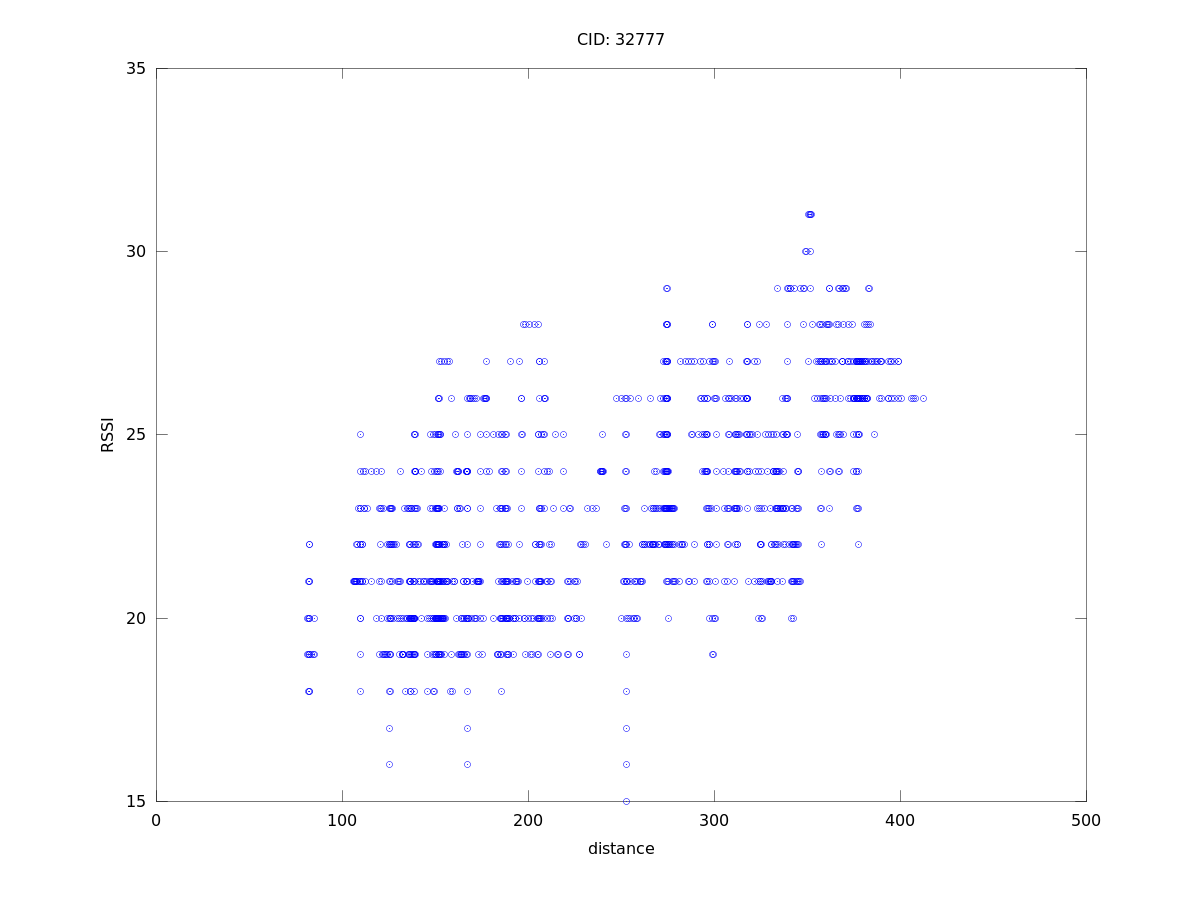
\includegraphics[width=1\textwidth]{cell32777raw.png}
		\end{subfigure}
		\begin{subfigure}[b]{0.3\textwidth}
			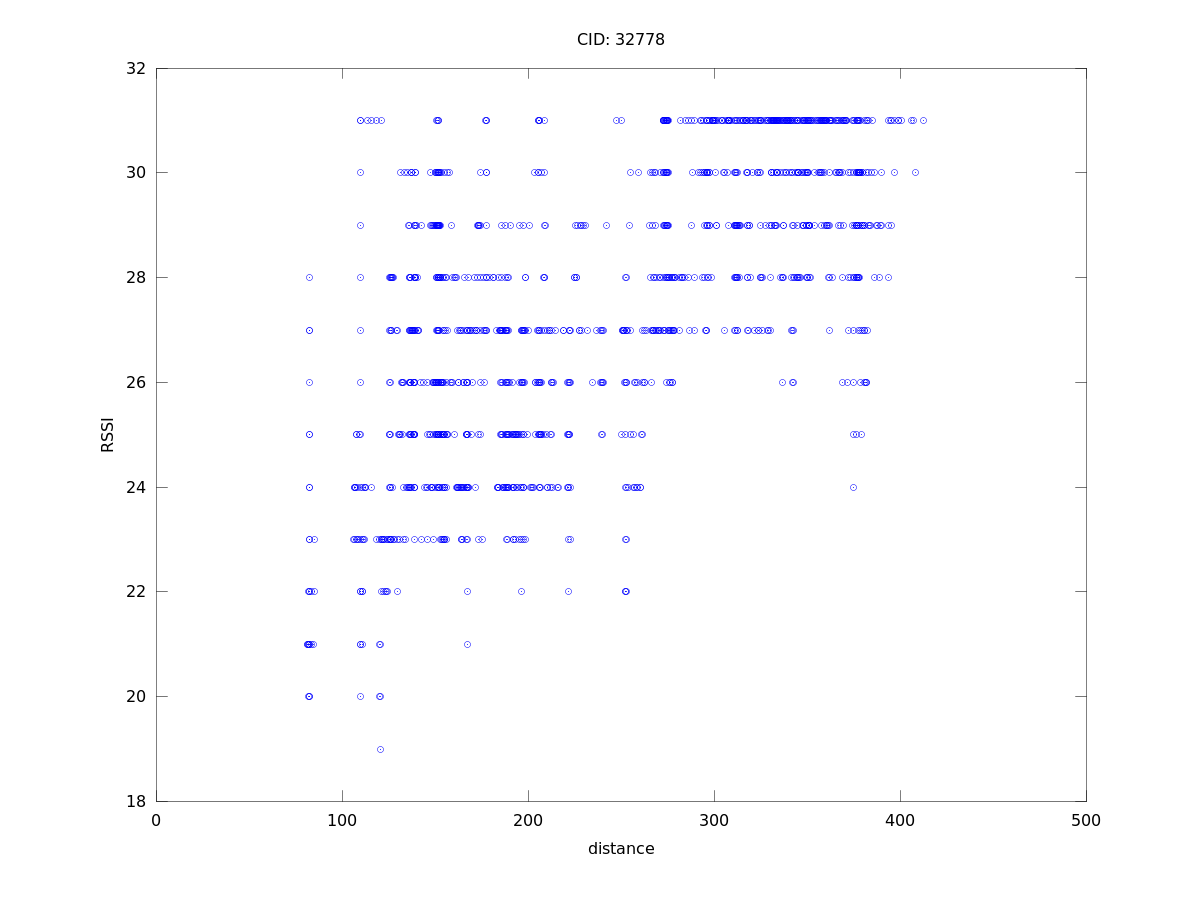
\includegraphics[width=1\textwidth]{cell32778raw.png}
		\end{subfigure}
		\begin{subfigure}[b]{0.3\textwidth}
			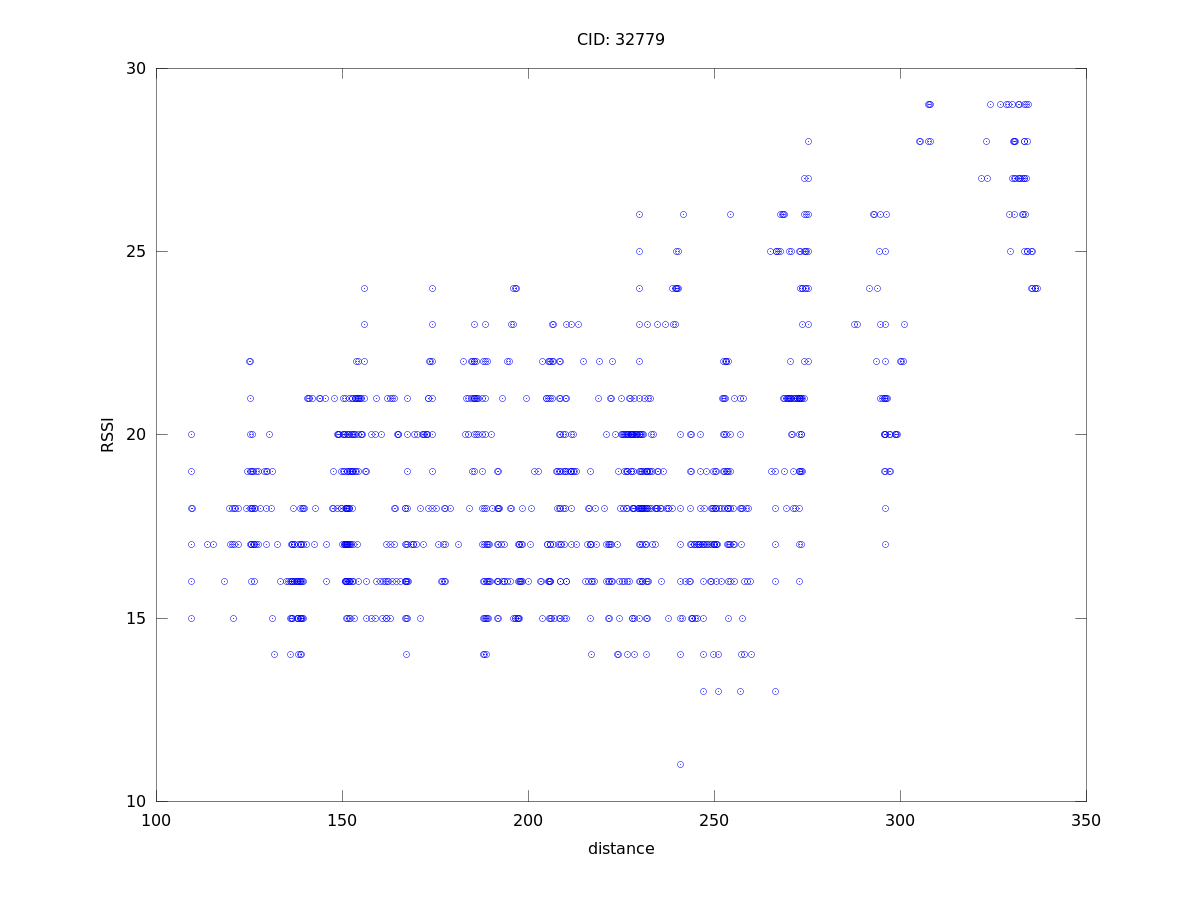
\includegraphics[width=1\textwidth]{cell32779raw.png}
		\end{subfigure}
	\end{center}
	\caption{Выборка данных для шести базовых станций, сигнал которых был принят позиционируемым устройством. Вертикальная ось --- asu, горизонтальная --- метры от начала маршрута.}
	\label{fig:exp-cell-raw}
\end{figure}

\subsection{Интерполяция}
\label{subsec:exp-interpol}
На данном этапе для выбранных множеств результатов предварительных замеров сигналов базовых станций строятся интерполяционные многочлены. На рис. \ref{fig:exp-cell-inter} приведены такие многочлены, степень каждого из которых определялась для каждой выборки индивидуально и равна одной десятой её длины. В пункте \ref{subsec:exp-order} вопрос выбора степени для интерполяционных многочленов рассмотрен более подробно.

\begin{figure}[p]
	\begin{center}
		\begin{subfigure}[b]{1\textwidth}
			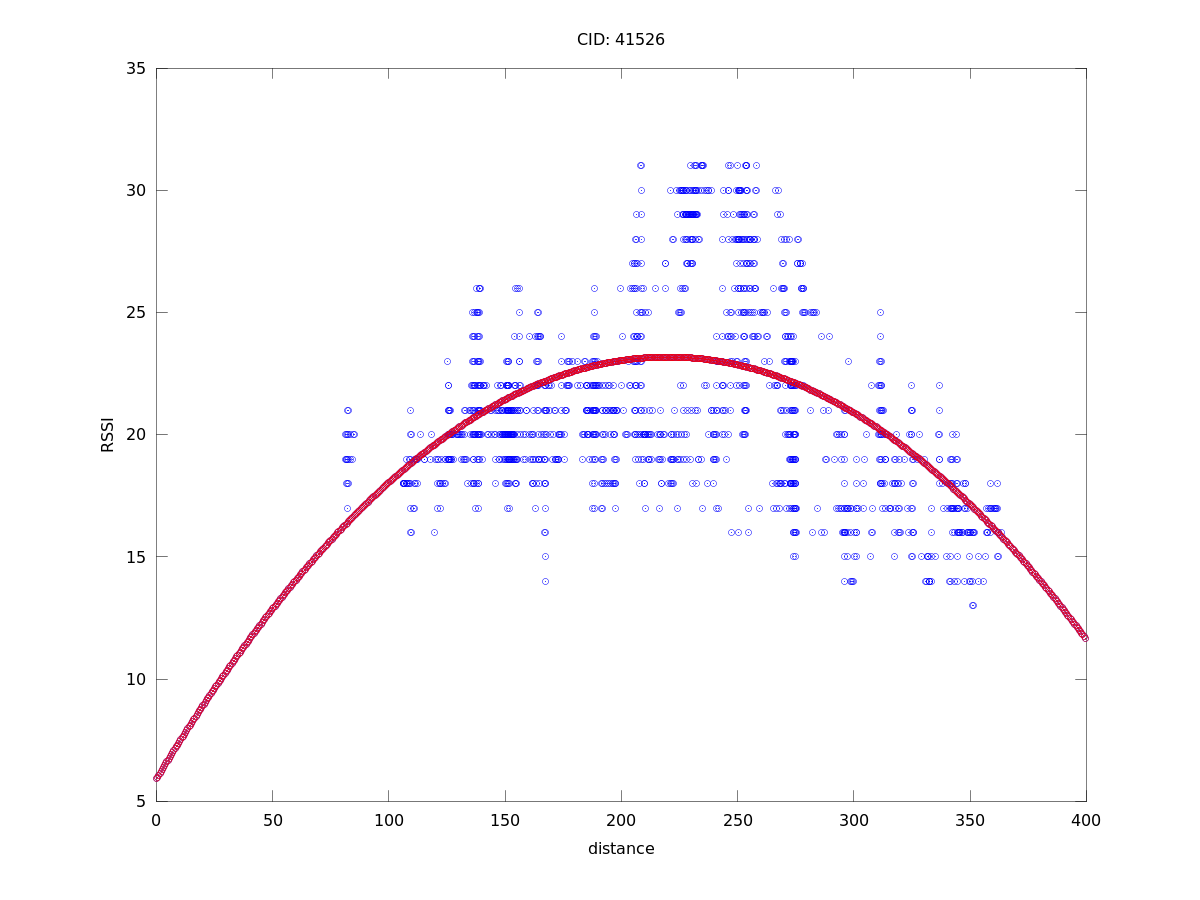
\includegraphics[width=1\textwidth]{cell41526inter.png}
		\end{subfigure}

		\begin{subfigure}[b]{0.45\textwidth}
			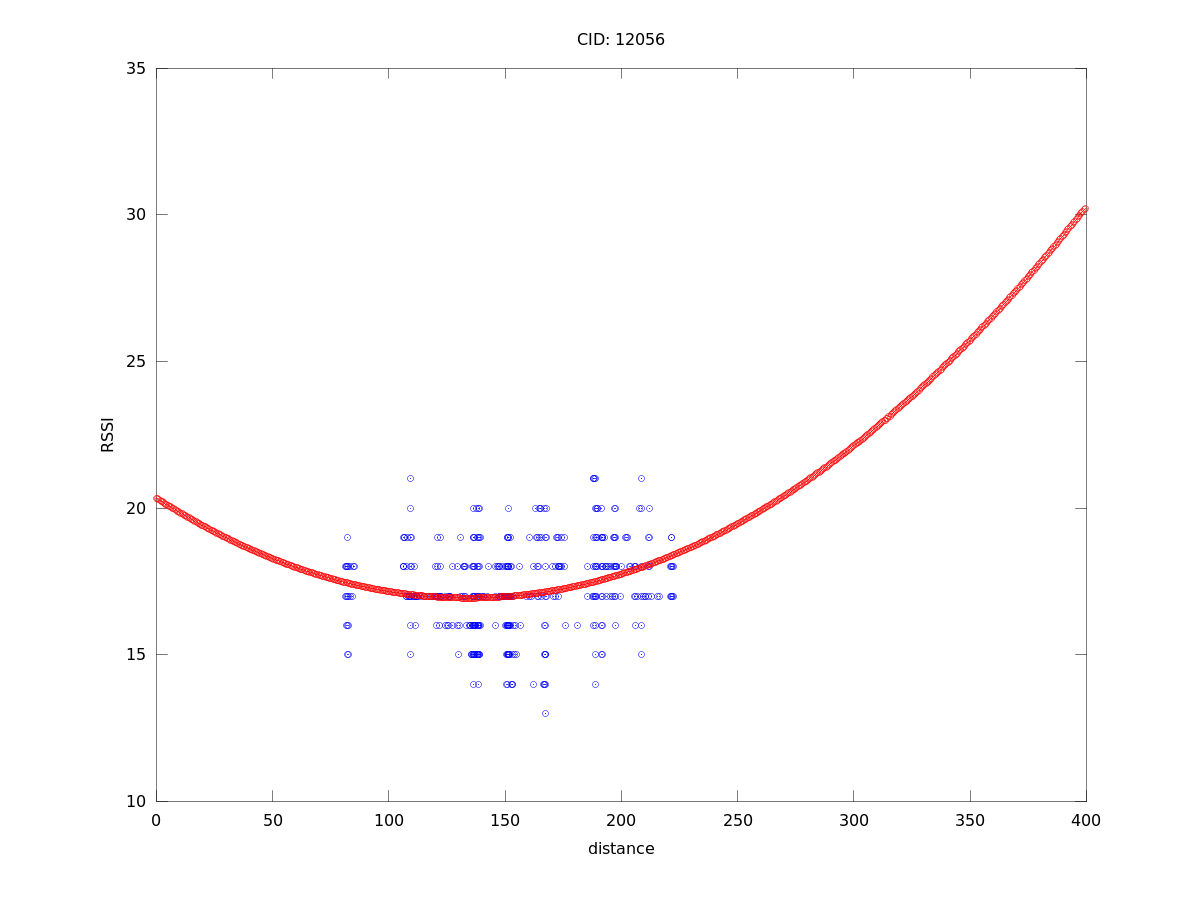
\includegraphics[width=1\textwidth]{cell12056inter.png}
		\end{subfigure}
		\begin{subfigure}[b]{0.45\textwidth}
			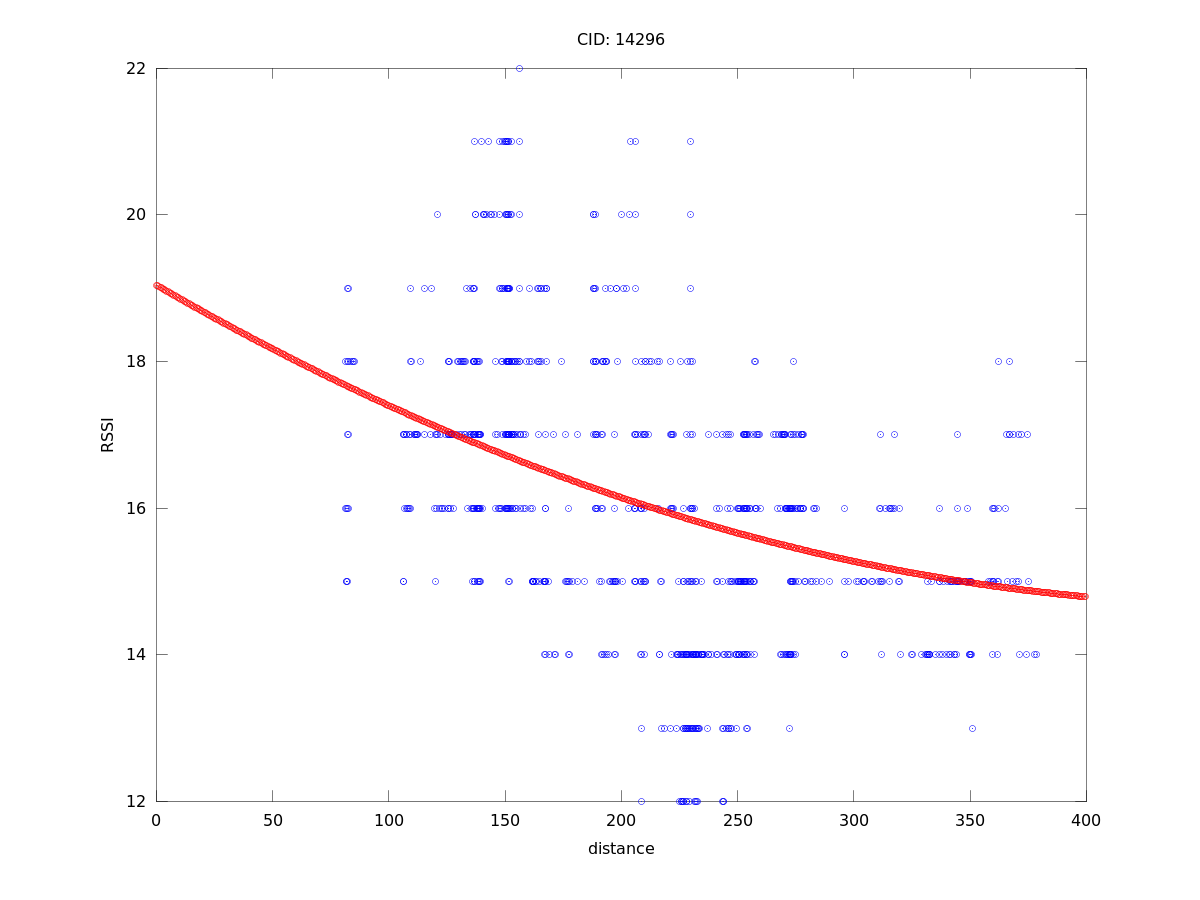
\includegraphics[width=1\textwidth]{cell14296inter.png}
		\end{subfigure}

		\begin{subfigure}[b]{0.3\textwidth}
			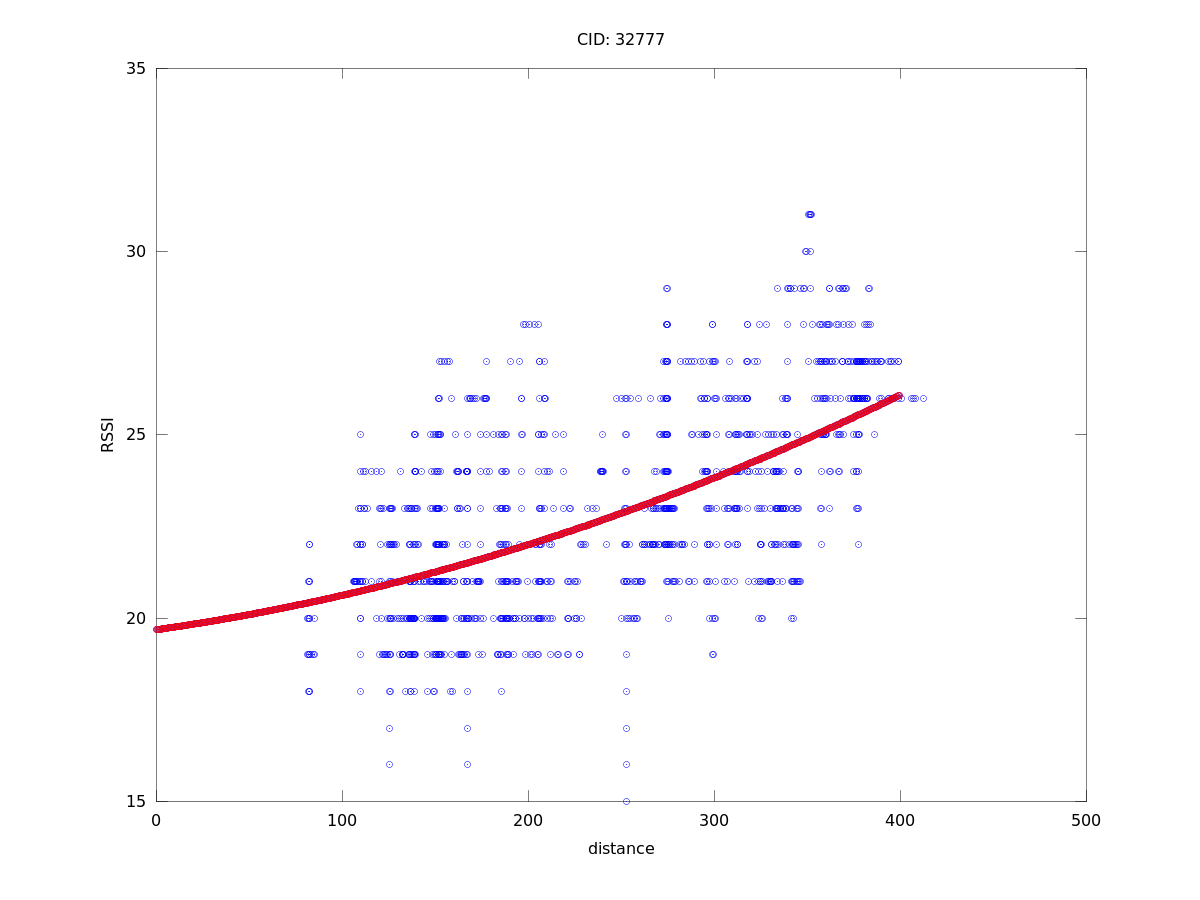
\includegraphics[width=1\textwidth]{cell32777inter.png}
		\end{subfigure}
		\begin{subfigure}[b]{0.3\textwidth}
			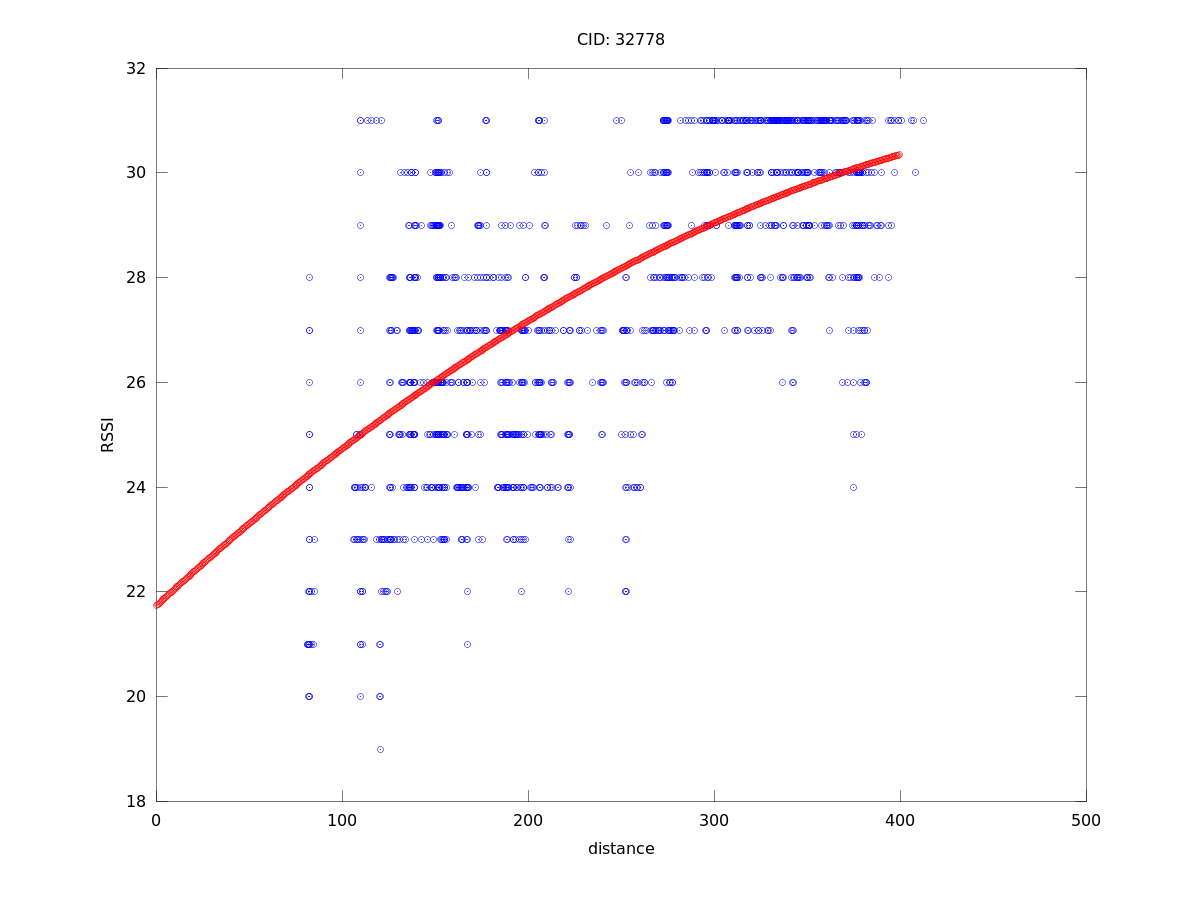
\includegraphics[width=1\textwidth]{cell32778inter.png}
		\end{subfigure}
		\begin{subfigure}[b]{0.3\textwidth}
			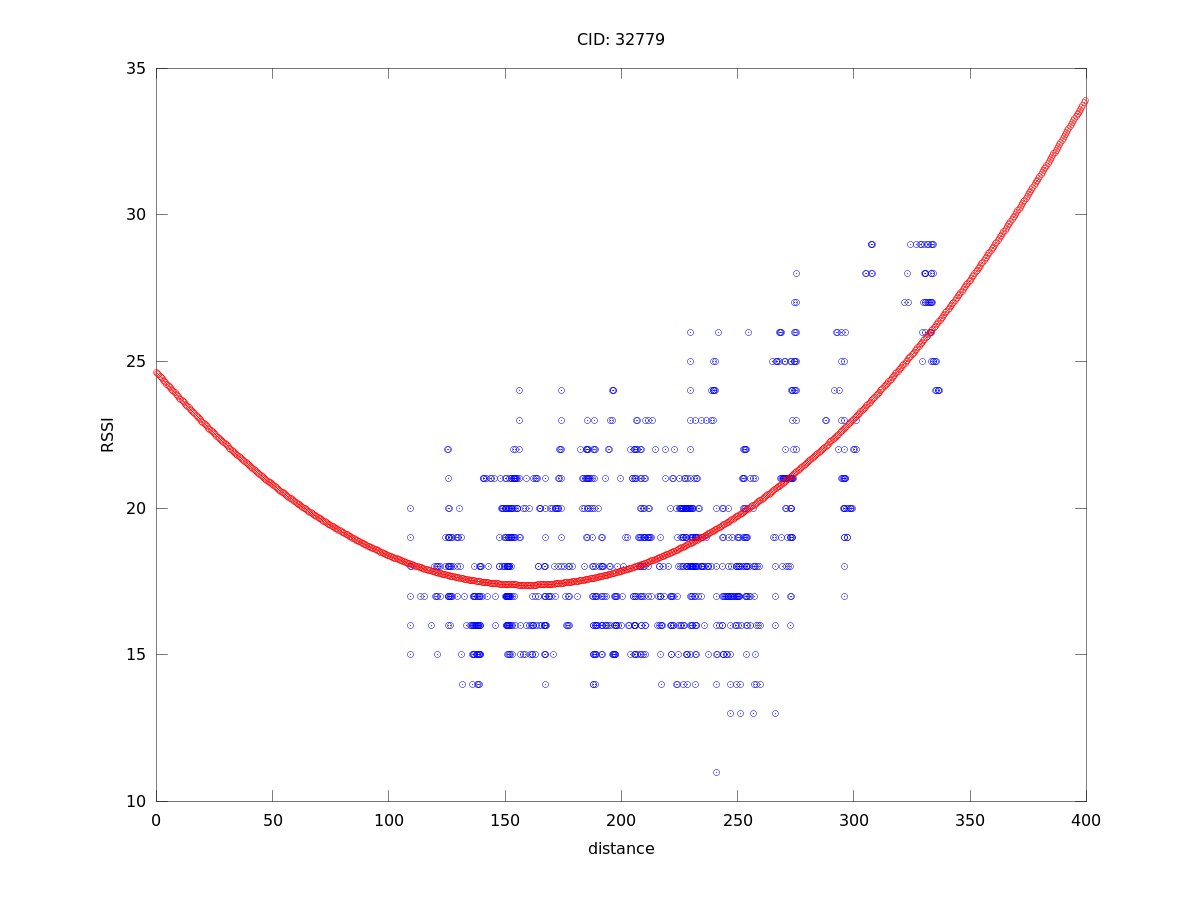
\includegraphics[width=1\textwidth]{cell32779inter.png}
		\end{subfigure}
	\end{center}
	\caption{Выборка данных о рассматриваемых станциях (точки) и интерполяционные многочлены для них (сплошные линии), полученные для степени, равной размерам выборок, делённым на 10. Вертикальная ось --- asu, горизонтальная --- метры от начала маршрута.}
	\label{fig:exp-cell-inter}
\end{figure}

\subsection{Псевдоплотности вероятности}

На данной стадии осуществляется сравнение статистических данных из базы, представленных в виде их интерполяционных многочленов, и фактически принятых RSSI. На рис. \ref{fig:exp-cell-pseudop} можно видеть, как приближение значения многочлена к фактически принятому ведёт к повышению значения псевдоплотности для данной точки.

\begin{figure}[p]
	\begin{center}
		\begin{subfigure}[b]{1\textwidth}
			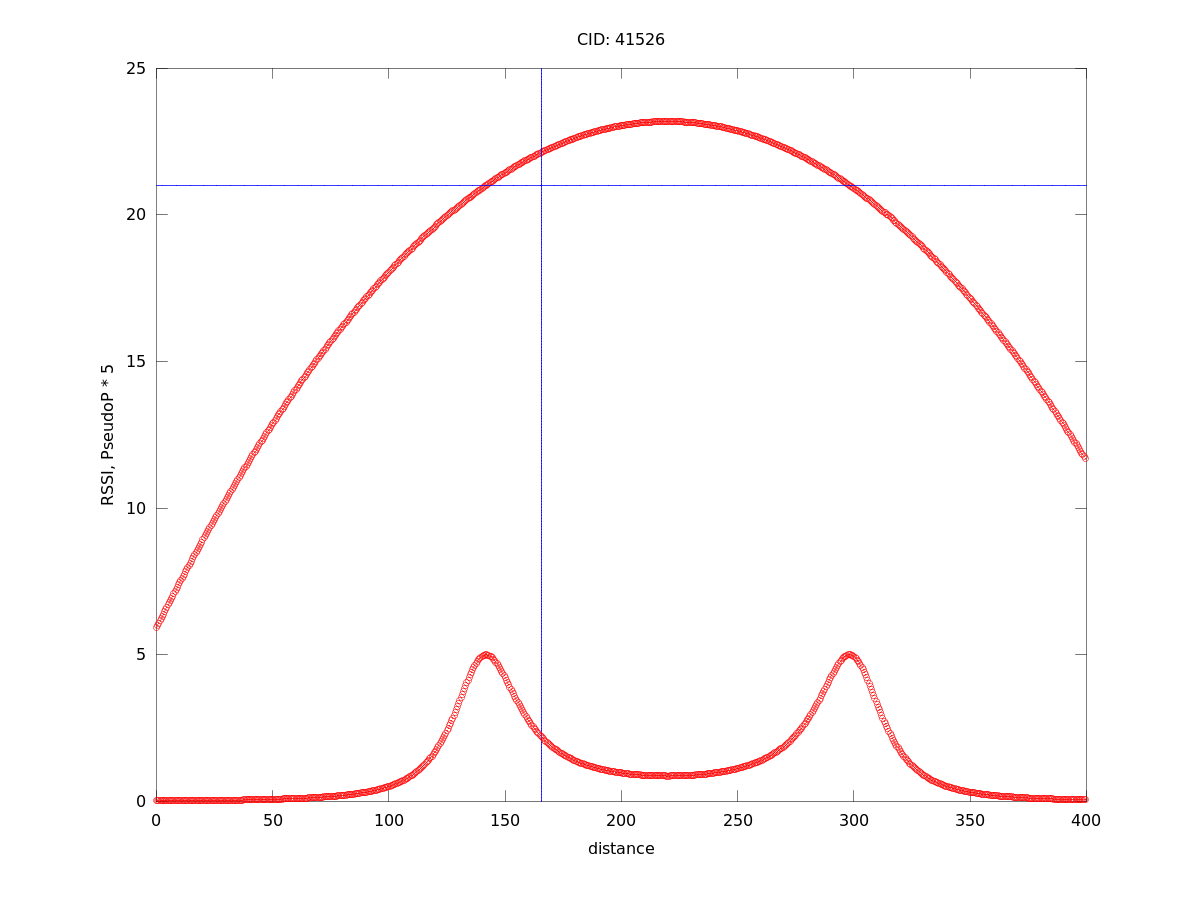
\includegraphics[width=1\textwidth]{cell41526pseudop.png}
		\end{subfigure}

		\begin{subfigure}[b]{0.4\textwidth}
			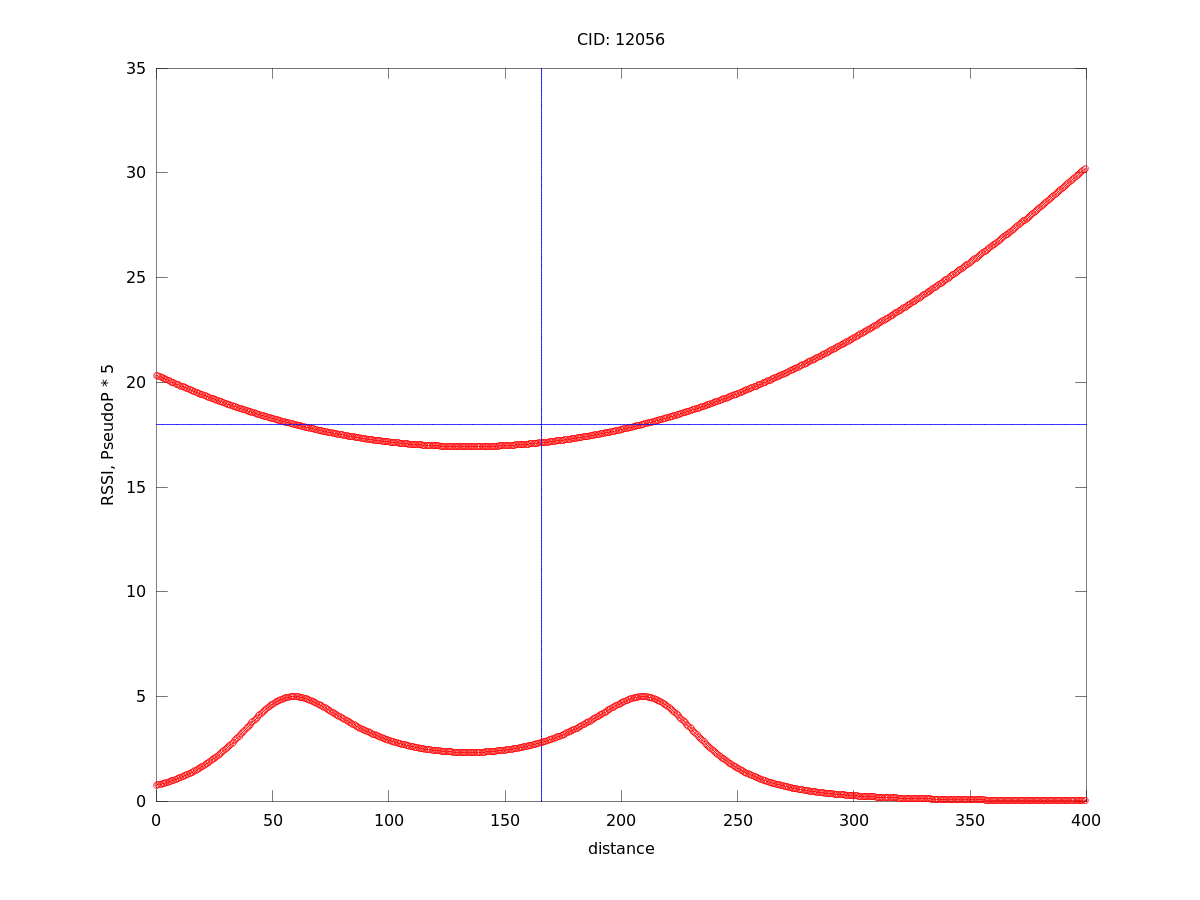
\includegraphics[width=1\textwidth]{cell12056pseudop.png}
		\end{subfigure}
		\begin{subfigure}[b]{0.4\textwidth}
			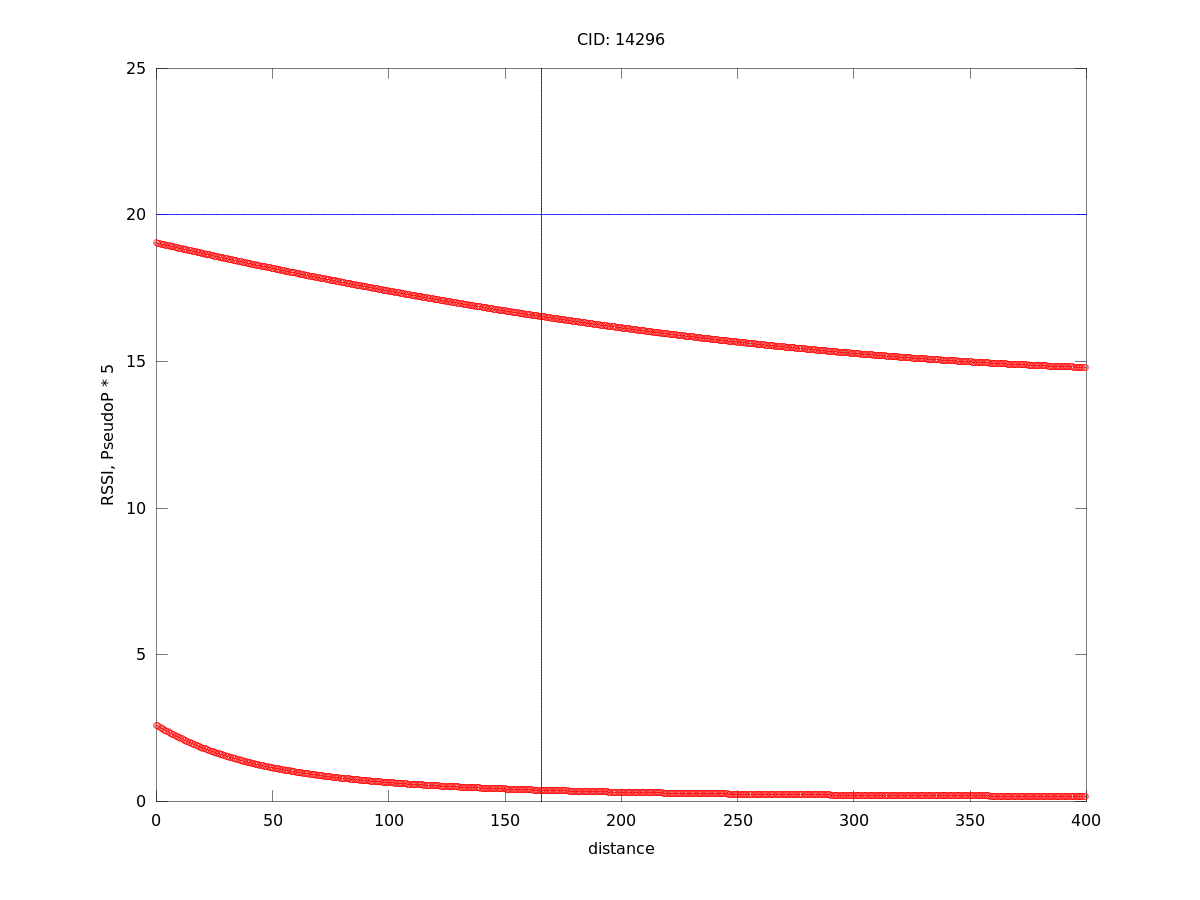
\includegraphics[width=1\textwidth]{cell14296pseudop.png}
		\end{subfigure}

		\begin{subfigure}[b]{0.25\textwidth}
			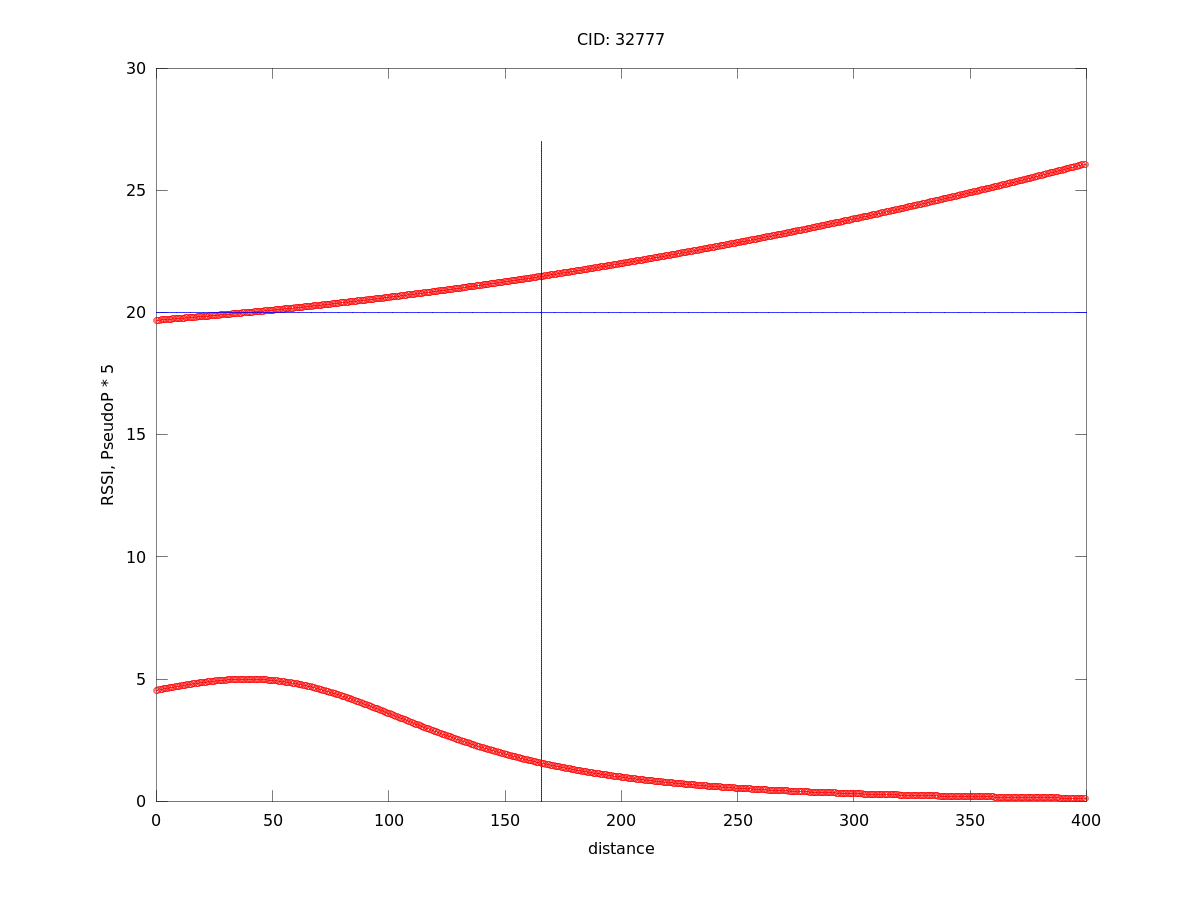
\includegraphics[width=1\textwidth]{cell32777pseudop.png}
		\end{subfigure}
		\begin{subfigure}[b]{0.25\textwidth}
			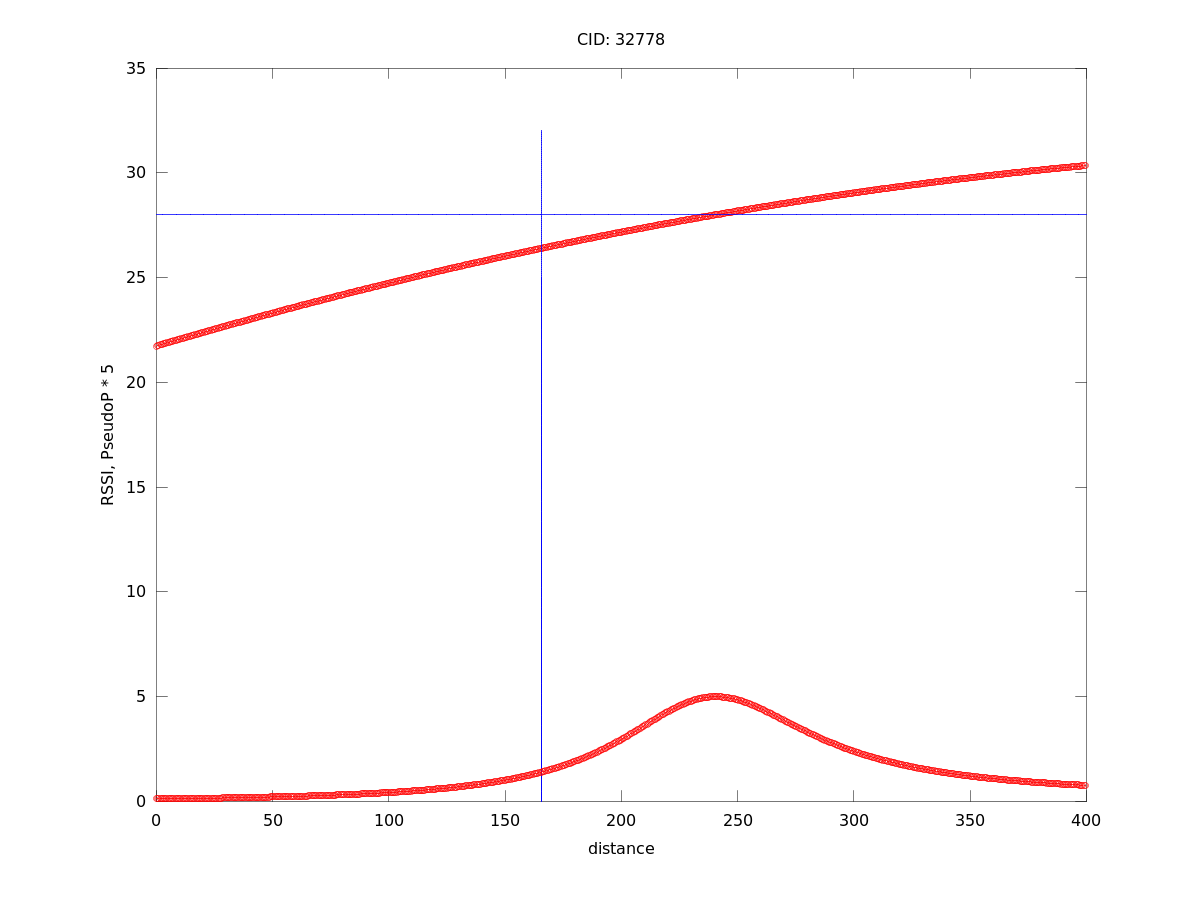
\includegraphics[width=1\textwidth]{cell32778pseudop.png}
		\end{subfigure}
		\begin{subfigure}[b]{0.25\textwidth}
			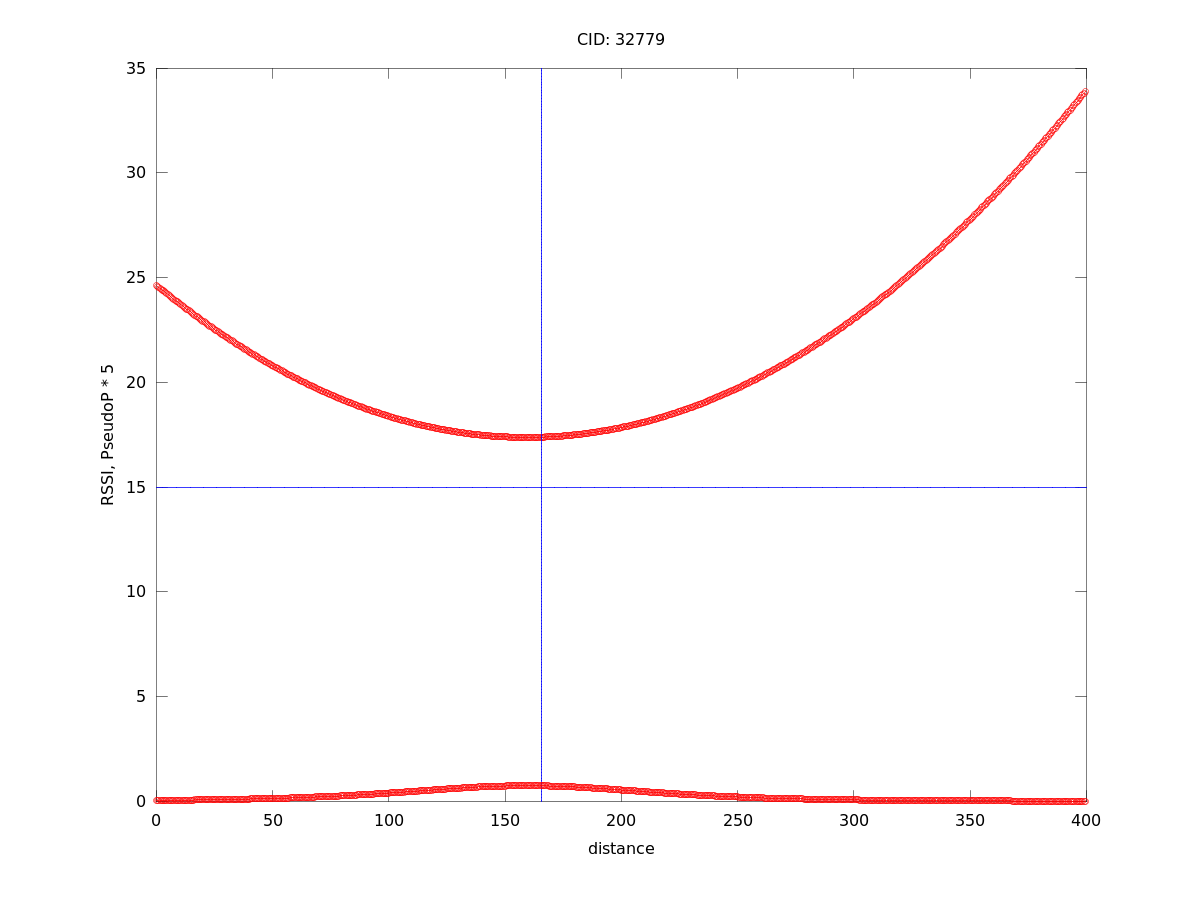
\includegraphics[width=1\textwidth]{cell32779pseudop.png}
		\end{subfigure}
	\end{center}
	\caption{Интерполяционные многочлены (толстая кривая сверху) и псевдоплотности вероятности (толстая кривая снизу) для принятых сигналов. Тонкая вертикальная прямая --- координата истинного положения, тонкая горизонтальная --- реально принятый RSSI для данной базовой станции. Вертикальная ось --- asu и единицы псевдоплотности, умноженные на 5, горизонтальная --- метры от начала маршрута.}
	\label{fig:exp-cell-pseudop}
\end{figure}

\subsection{Результирующая псевдоплотность}
\begin{figure}[h]
	\center{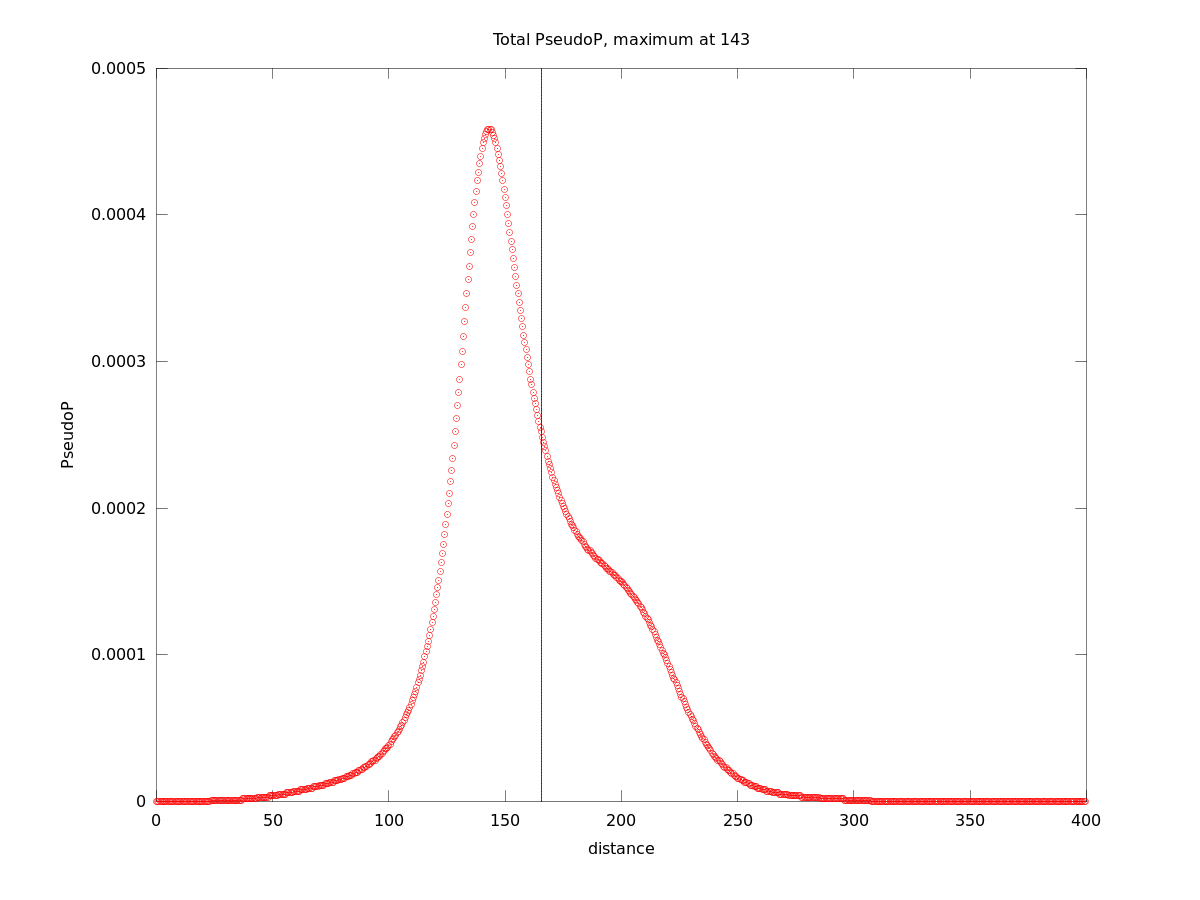
\includegraphics[width=1\linewidth]{totalpseudop.png}}
	\caption{Значения псевдоплотности в дискретно расположенных точках, обрабатывавшихся при поиске максимума. Вертикальная линия --- координата истинного положения устройства. Вертикальная ось --- единицы псевдоплотности, горизонтальная --- метры. Аргумент максимального положения --- 143 метра.}
	\label{fig:totalpseudop}
\end{figure}

Последний оставшийся шаг --- это перемножение независимо посчитанных псевдоплотностей для разных базовых станций между собой и поиск аргумента максимума полученной функции. На рис. \ref{fig:totalpseudop} изображена эта функция. Аргумента её максимума --- 143 метра, реальное положение устройства по данным GPS --- 165,5 метров. Итоговая ошибка составила 22,5 метров.

\section{Погрешность}
Перейдя от рассмотрения однократного процесса поиска местонахождения устройства к статистике этого процесса, рассмотрим, какое значение ошибки является типичным для реализованного алгоритма в условиях поставленного эксперимента.

\begin{figure}[h]
	\center{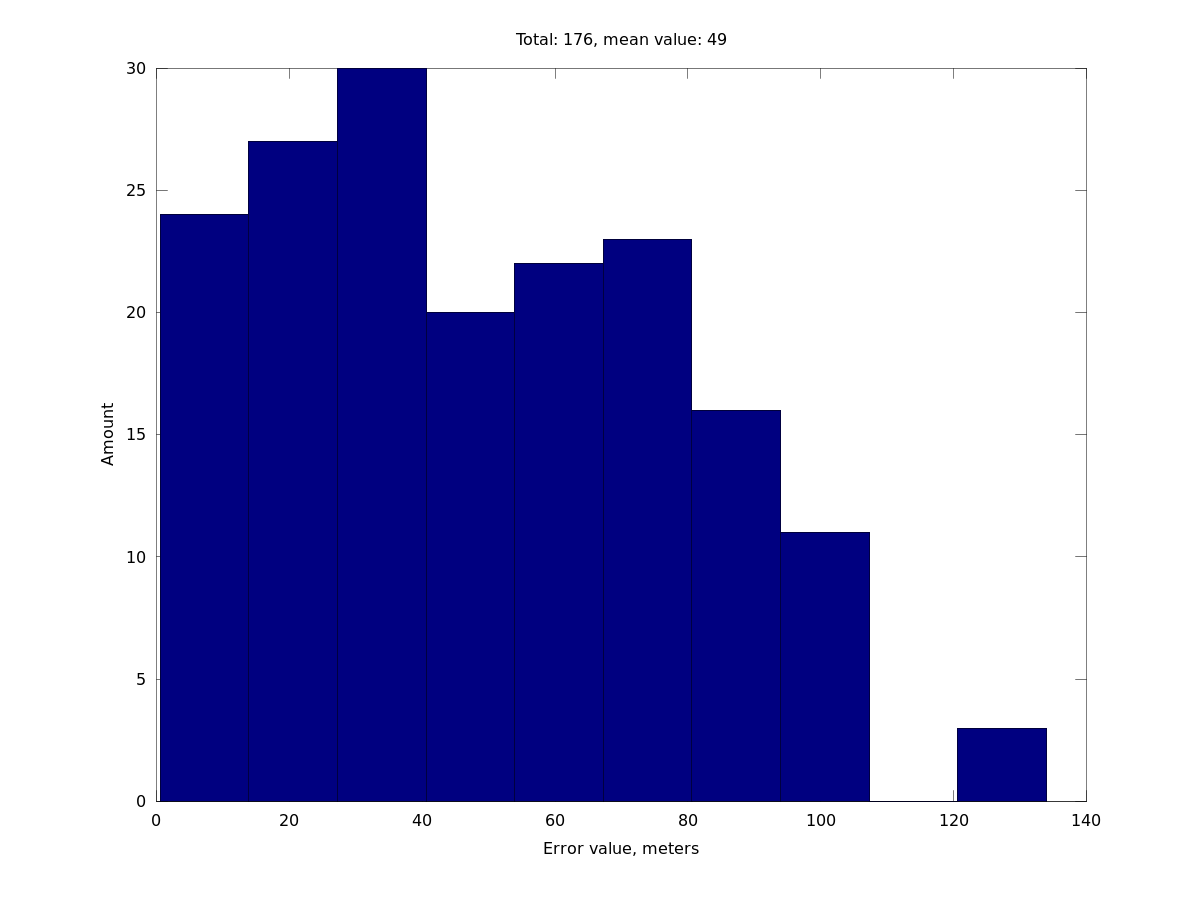
\includegraphics[width=1\linewidth]{errhist.png}}
	\caption{Гистограмма величин ошибок позиционирования. Горизонтальная ось --- величина ошибки в метрах, вертикальная --- количество появлений такой ошибки в экспериментах. Всего 176 примеров, математическое ожидание ошибки --- 49 метров.}
	\label{fig:errhist}
\end{figure}

Было поставлено 176 экспериментов, по возможности распределённых равномерно по всей длине маршрута. Для каждого из них отмечалось истинное значение расстояния от начала маршрута и результат его вычисления на основе данных GSM. После этого было вычислено расстояние между истинным и рассчитанным положением. Гистограмма полученной выборки изображена на рис. \ref{fig:errhist}. Математическое ожидание ошибки составило 49 метров.

\section{Анализ экспериментальных данных}

Точность позиционирования, достигнутая в ходе экспериментов, превышает современные системы, основанные на триангуляционном методе, но ещё не достигает точности спутниковых систем, что было бы идеальным результатом. Рассмотрим, какие факторы могут стоять на пути к повышению точности.

\subsection{Степени интерполяционных многочленов}
\label{subsec:exp-order}
Самый заметный из факторов видно на рис. \ref{fig:exp-cell-pseudop} --- очень простой вид полученных интерполяционных многочленов. Все они либо имеют лишь один видимый экстремум, либо позволяют предположить его наличие за пределами графиков (поскольку конечный многочлен с положительными степенями асимптотически сходиться к какому-либо конечному числу на может). Изначальная гипотеза предполагала наличие более сложного вида этой зависимости, который бы привёл к более выраженным экстремумам функции псевдоплотности вероятности и позволил достигнуть большей точности.

Проанализируем, с чем это может быть связано. В ходе процесса построения многочленов, описанного в пункте \ref{subsec:exp-interpol}, в качестве максимальной степени для каждого многочлена выбиралось значение, разное одной десятой размера выборки. Для разных базовых станций размеры выборок различаются, начинаясь от десятков замеров и заканчиваясь тысячами. Таким образом, и степени многочленов получаются существенным образом разные.

\begin{figure}[h]
	\begin{center}
		\begin{subfigure}[b]{0.45\textwidth}
			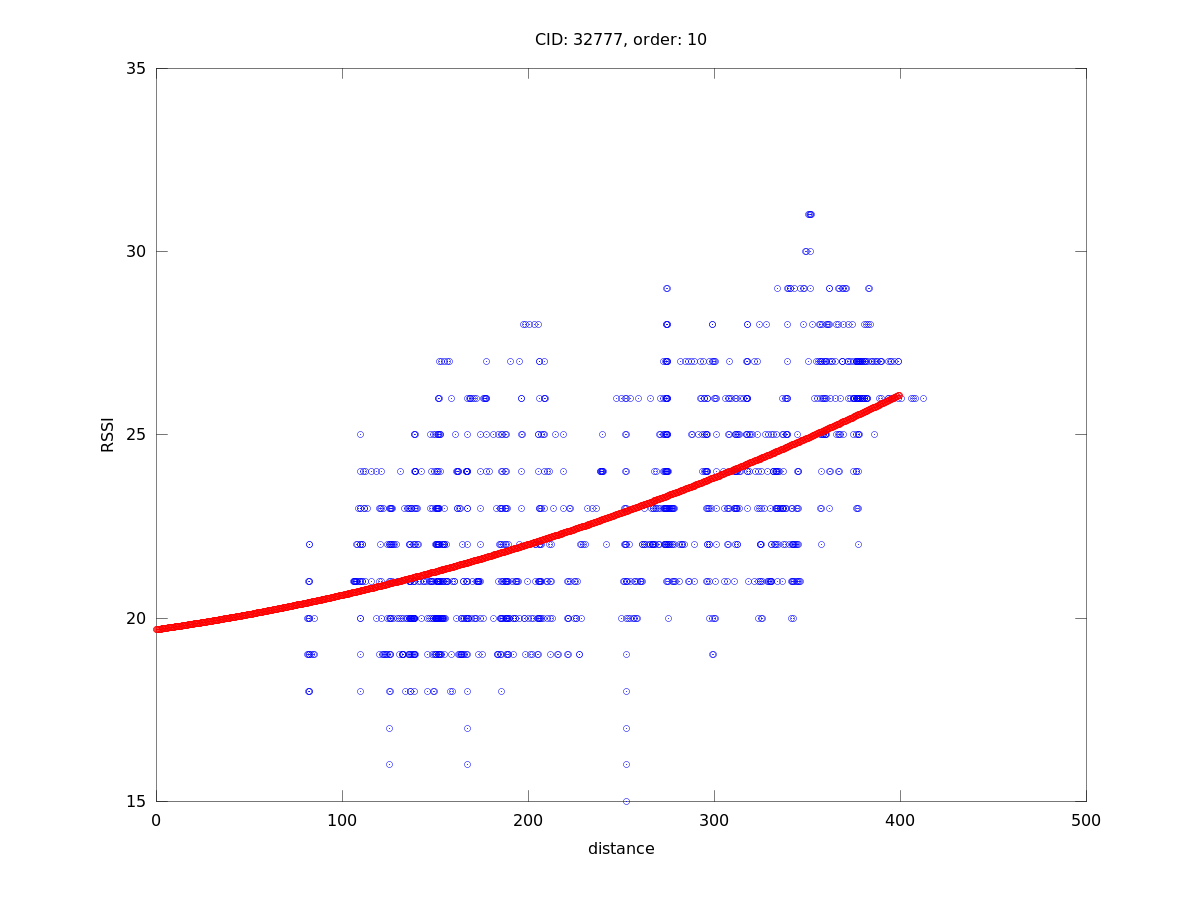
\includegraphics[width=1\textwidth]{cell32777inter10.png}
			\caption{Максимальная степень --- 10.}
		\end{subfigure}
		\begin{subfigure}[b]{0.45\textwidth}
			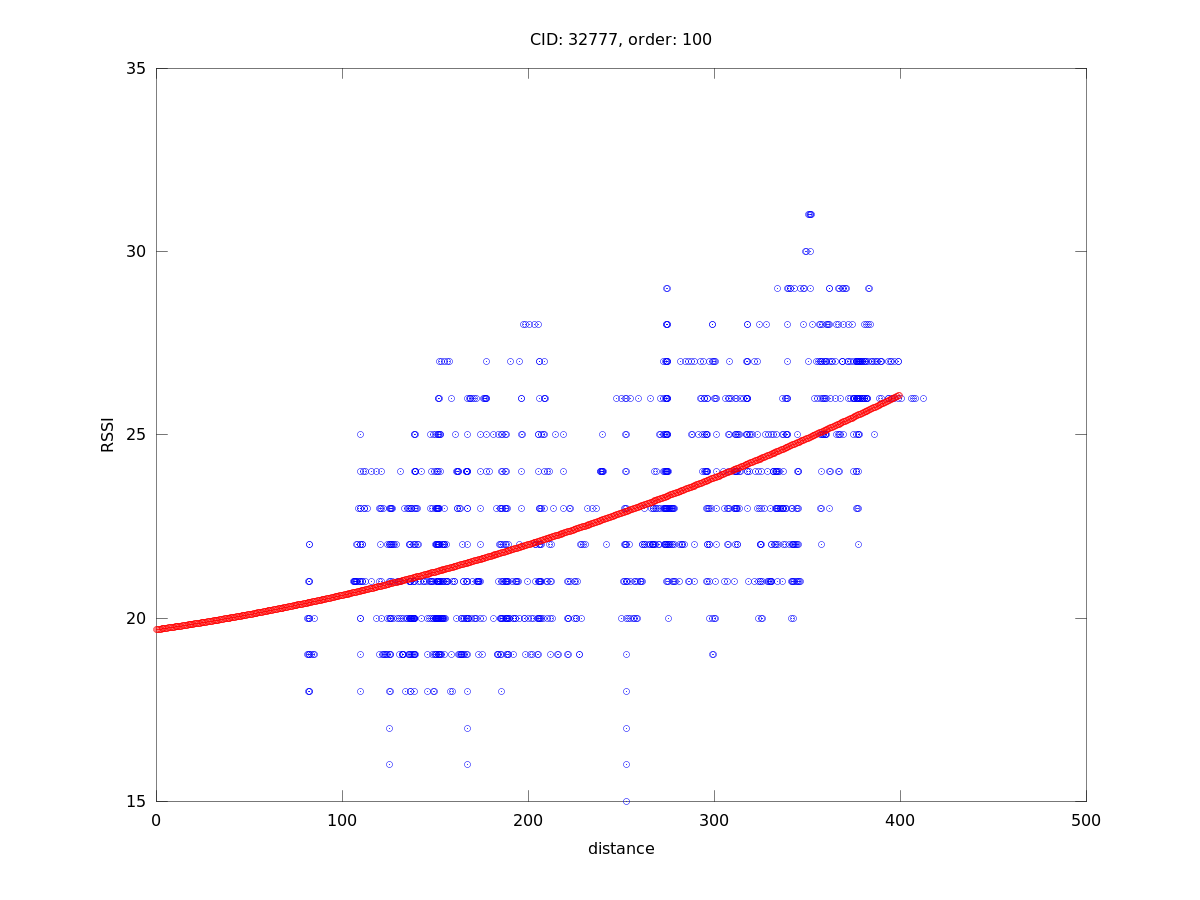
\includegraphics[width=1\textwidth]{cell32777inter100.png}
			\caption{Максимальная степень --- 100.}
		\end{subfigure}
	\end{center}
	\caption{Вид интерполяционных многочленов для выборки базовой станции 32777 при разной степени. Вертикальная ось --- asu, горизонтальная --- метры от начала маршрута.}
	\label{fig:exp-cell-order}
\end{figure}
Возьмём одну конкретную базовую станцию, пусть это будет 32777, для которой в базе имеется 2953 замеров, и построим для неё интерполяционные многочлены с разными степенями. На рис. \ref{fig:exp-cell-order} показаны интерполяционные многочлены десятой и сотой степени --- разницы между ними нет. Таким образом получается, что полученные в пункте \ref{subsec:exp-interpol} многочлены действительно являются лучшими полиномиальными приближениями имеющихся массивов данных (причём стоит отметить, что на отрезке 400 метров многочлен сотой степени может с большой точностью приблизить практически любую зависимость, имеющую физический смысл).

\subsection{Возможные дальнейшие эксперименты}
Итак, зависимость уровня от сигнала от расстояния до станции, выявленная в ходе экспериментов, имеет вид, отличающийся от теоретического предсказания, но имеет простой вид, а не обладает множеством экстремумов, порождённых отражениями сигнала, поглощением городской застройкой и прочими систематическими факторами. В связи с этим, важным вопросом, который должен быть выяснен в ходе дальнейших экспериментов, является такой: действительно ли погрешности носят преимущественно случайный характер, и в ходе экспериментов была выявлена единственная систематически наблюдаемая закономерность?

Одним из таких экспериментов видится следующий: сравнение статистических данных об уровнях сигнала в ряде точек с учётом и без учёта соседних. При многократных изменениях на первый план должны выйти именно постоянные факторы, а не случайные. Таким образом, если во многих точках, распределённых по маршруту, средние результаты многократных измерений будут сходиться к интерполяционному многочлену, даже несмотря на то, что измерения усредняются только по одной точке, в многочлен учитывает все, это будет сильным аргументом в пользу того, что выявленные зависимости являются единственными. И, следовательно, полученная точность близка к теоретическому пределу точности позиционирования, которую можно получить в сотовых сетях.

Если же такой сходимости наблюдаться не будет, это будет означать, что статистические методы как таковые могут работать точнее, но необходимо работать над совершенствованием методов, чтобы выявить дополнительные скрытые закономерности.
